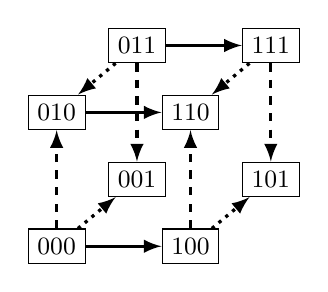
\begin{tikzpicture}
	\tikzstyle{stgstate} = [draw,font=\small]
	\tikzstyle{stgedge} = [-latex,very thick,font=\sffamily\normalsize\bfseries]

	\def\incx{1.7}
	\def\incy{1.7}
	\colorlet{darkgreen}{green!50!black}

	% NODES %
	\node[stgstate] (000) at (0*\incx,0*\incy) {000};
	\node[stgstate] (100) at (1*\incx,0*\incy) {100};
	\node[stgstate] (001) at (0.6*\incx,0.5*\incy) {001};
	\node[stgstate] (101) at (1.6*\incx,0.5*\incy) {101};

	\node[stgstate] (010) at (0*\incx,1*\incy) {010};
	\node[stgstate] (110) at (1*\incx,1*\incy) {110};
	\node[stgstate] (011) at (0.6*\incx,1.5*\incy) {011};
	\node[stgstate] (111) at (1.6*\incx,1.5*\incy) {111};

	% EDGES %
	%g1
	\draw[stgedge] (000) edge (100);
	\draw[stgedge] (010) edge (110);
	\draw[stgedge] (011) edge (111);
	%g2
	\draw[stgedge,dashed] (000) edge (010);
	\draw[stgedge,dashed] (100) edge (110);
	\draw[stgedge,dashed] (011) edge (001);
	\draw[stgedge,dashed] (111) edge (101);
	%g3
	\draw[stgedge,dotted] (000) edge (001);
	\draw[stgedge,dotted] (100) edge (101);
	\draw[stgedge,dotted] (011) edge (010);
	\draw[stgedge,dotted] (111) edge (110);
\end{tikzpicture}
